\section{k-means segmentation}

We can see in figures \ref{fig:animals-k5-no-spatial} and
\ref{fig:animals-k10-no-spatial} the result of segmenting
the image \texttt{animals.jpg} with k-means with K=5 and K=10, respectively.
The K parameter denotes the number of different clusters (i.e. regions in
which the image is segmented). No transformations have been applied up to this point.

Whether the results are satisfactory or not depends on the application.
If, for instance, we wish to separate the animals from the
background we would like that the labels assigned to the
pixels that belong to the animals are different than those
assigned to the vegetation that surrounds them. Should this
be case it turns out that with K=5 some pixels from the
animals are assigned labels that correspond to the background
(check the primate and the tigers).

On the other hand K=10 does a better job distinguishing the
animals from the background, although (arguably) at the price
of having some over-segmentation (the unnecessary distinction
between different shades of the animals hair).

In both cases we can see that the assignment of labels to the lion
and the grass is somewhat erratic and noisy. This is due to the texture
of those regions. We will see later that this phenomenon can be counteracted
by means of scaling down (losing image details), by taking into account the
spatial coordinates of each pixel, or doing both.

It is also worth
mentioning how the algorithm can have artistic purposes, serving as
a technique to achieve the
`posterization' effect present in some photographic suites such as GIMP
or Photoshop.

\begin{figure}[hbt]
\centering
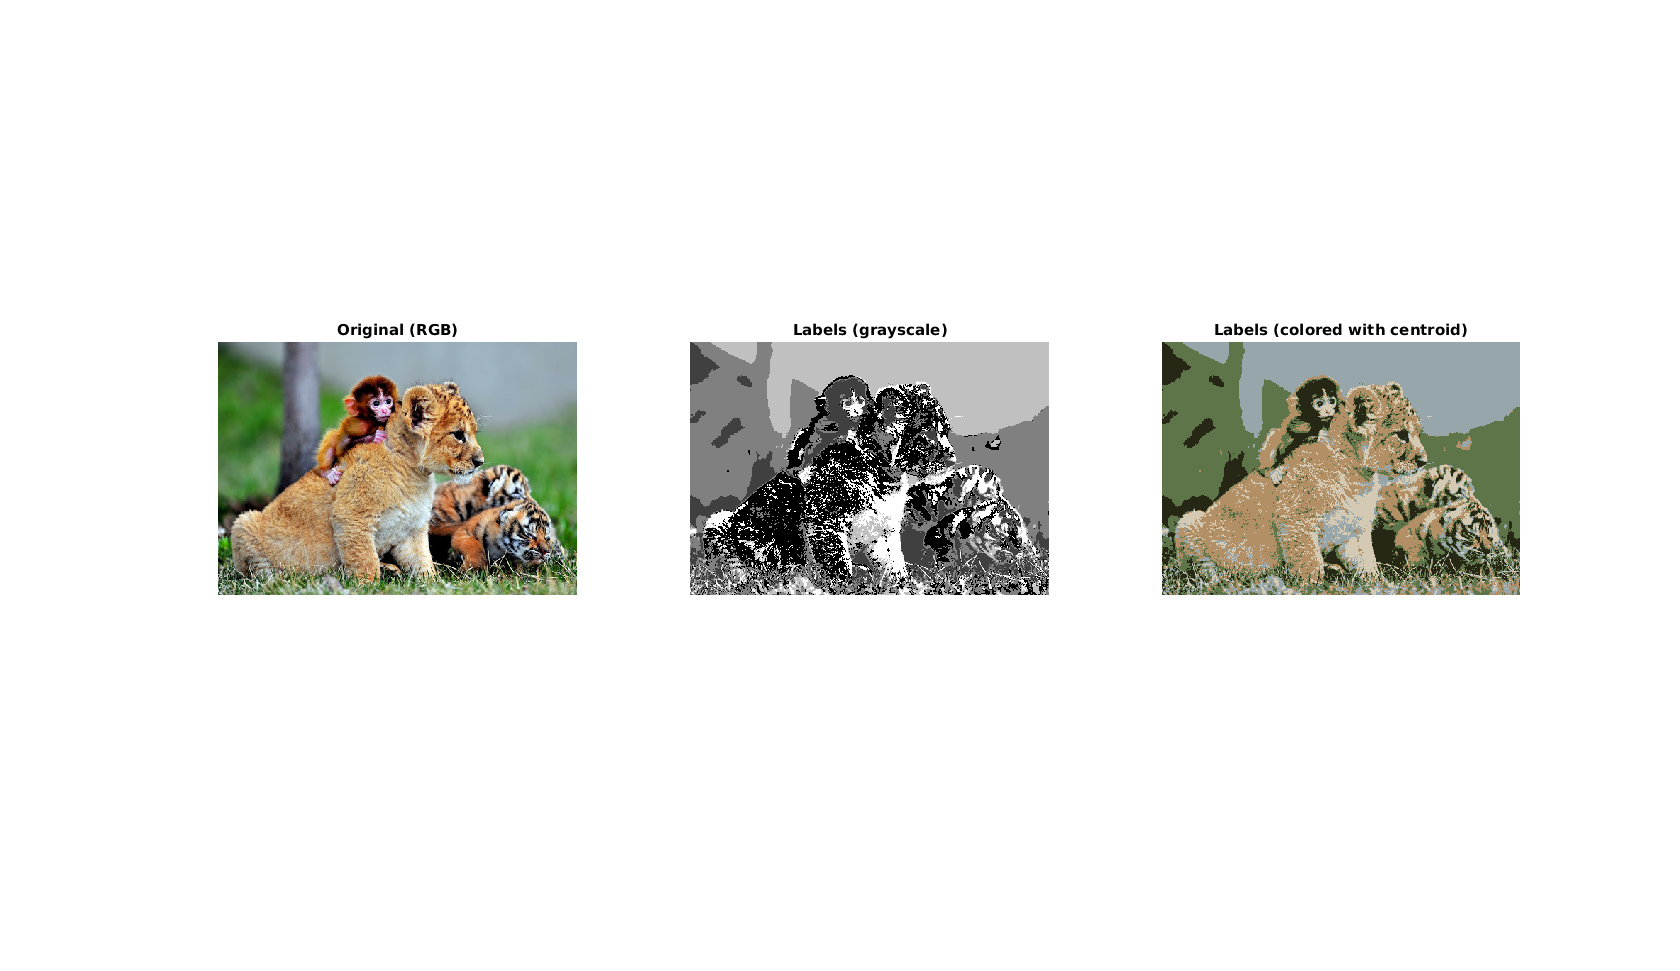
\includegraphics[trim={50px 250px 50px 220px},clip,width=\textwidth]{img/kmeans/animals_k5_no_spatial.png}
\caption{Segmentation of \texttt{animals.jpg} with K-means (K = 5)}
\label{fig:animals-k5-no-spatial}
\end{figure}

\begin{figure}[hbt]
\centering
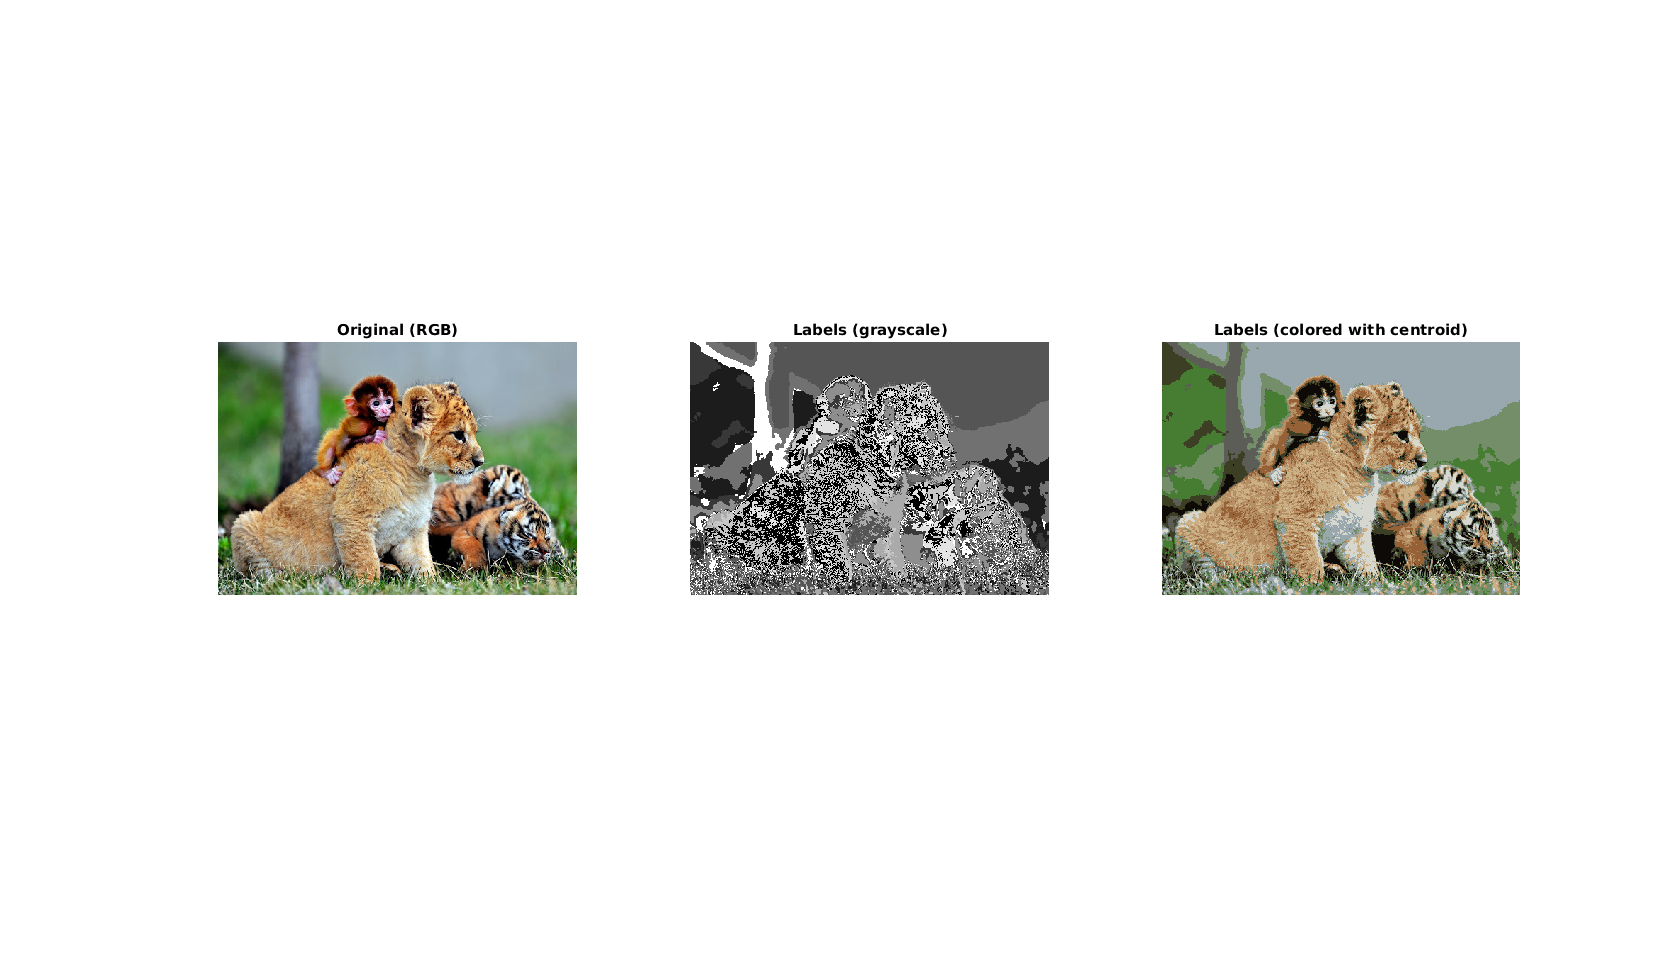
\includegraphics[trim={50px 250px 50px 220px},clip,width=\textwidth]{img/kmeans/animals_k10_no_spatial.png}
\caption{Segmentation of \texttt{animals.jpg} with K-means (K = 10)}
\label{fig:animals-k10-no-spatial}
\end{figure}

We can see more results for other images in figures \ref{fig:bigbangfamily-k8-no-spatial}
and \ref{fig:alwin2-k8-no-spatial}.

\begin{figure}[hbt]
\centering
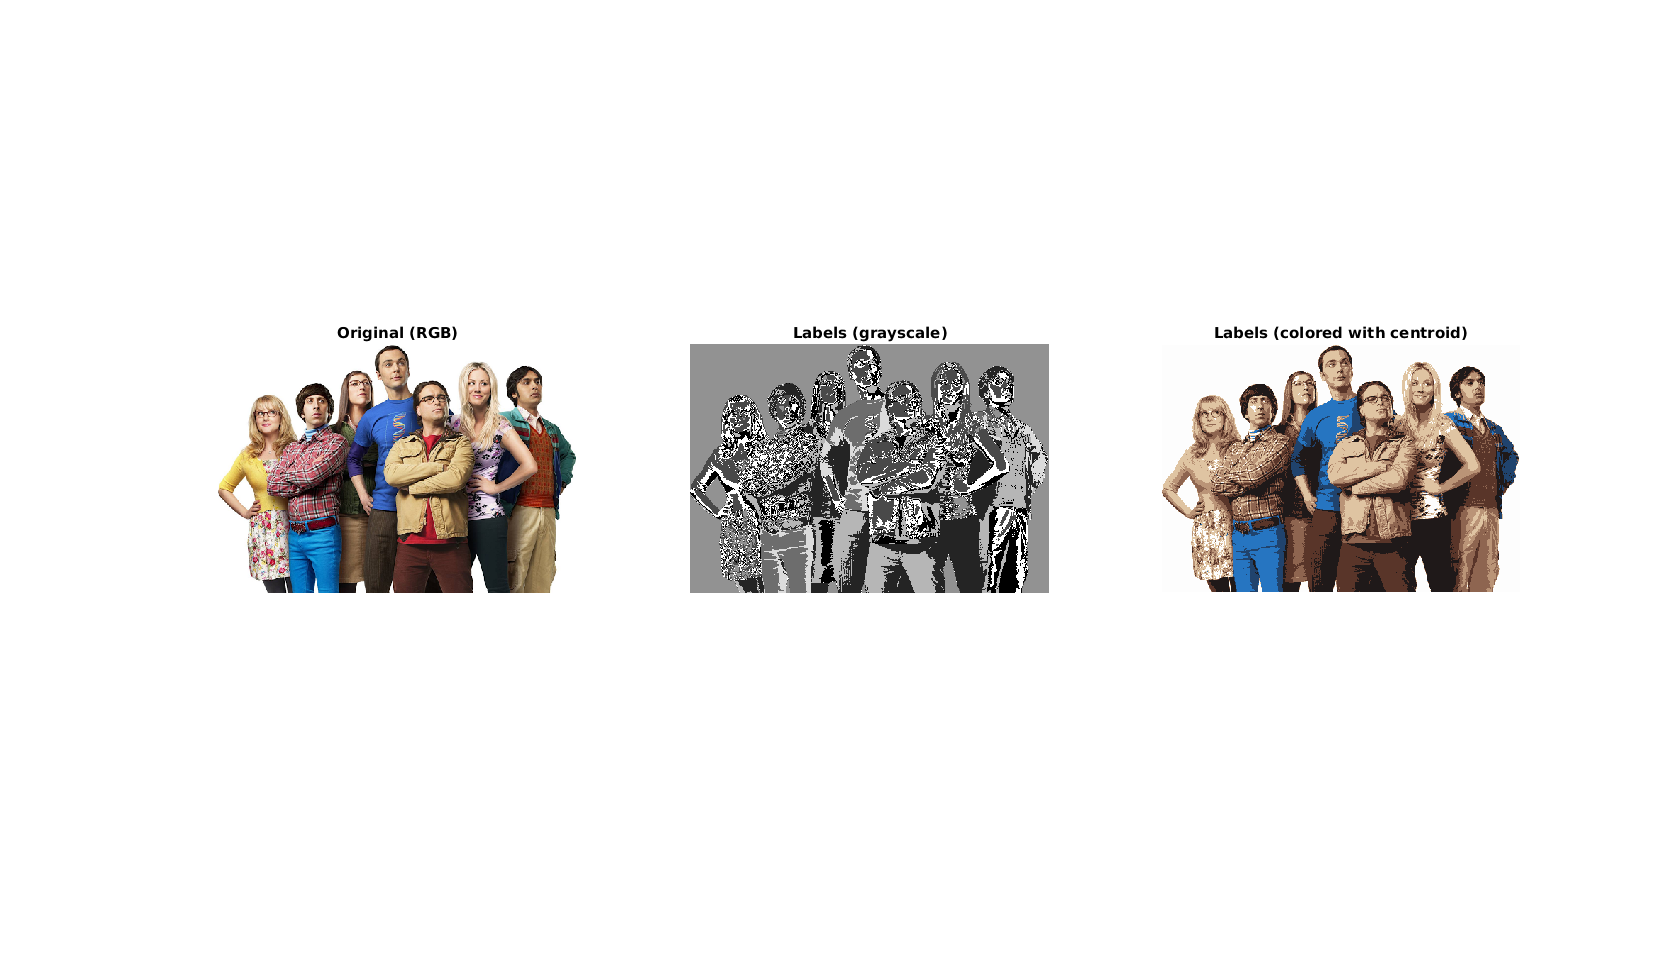
\includegraphics[trim={50px 250px 50px 220px},clip,width=\textwidth]{img/kmeans/bigbangfamily_k8_no_spatial.png}
\caption{Segmentation of \texttt{bigbangfamily.png} with K-means (K = 8)}
\label{fig:bigbangfamily-k8-no-spatial}
\end{figure}

\begin{figure}[hbt]
\centering
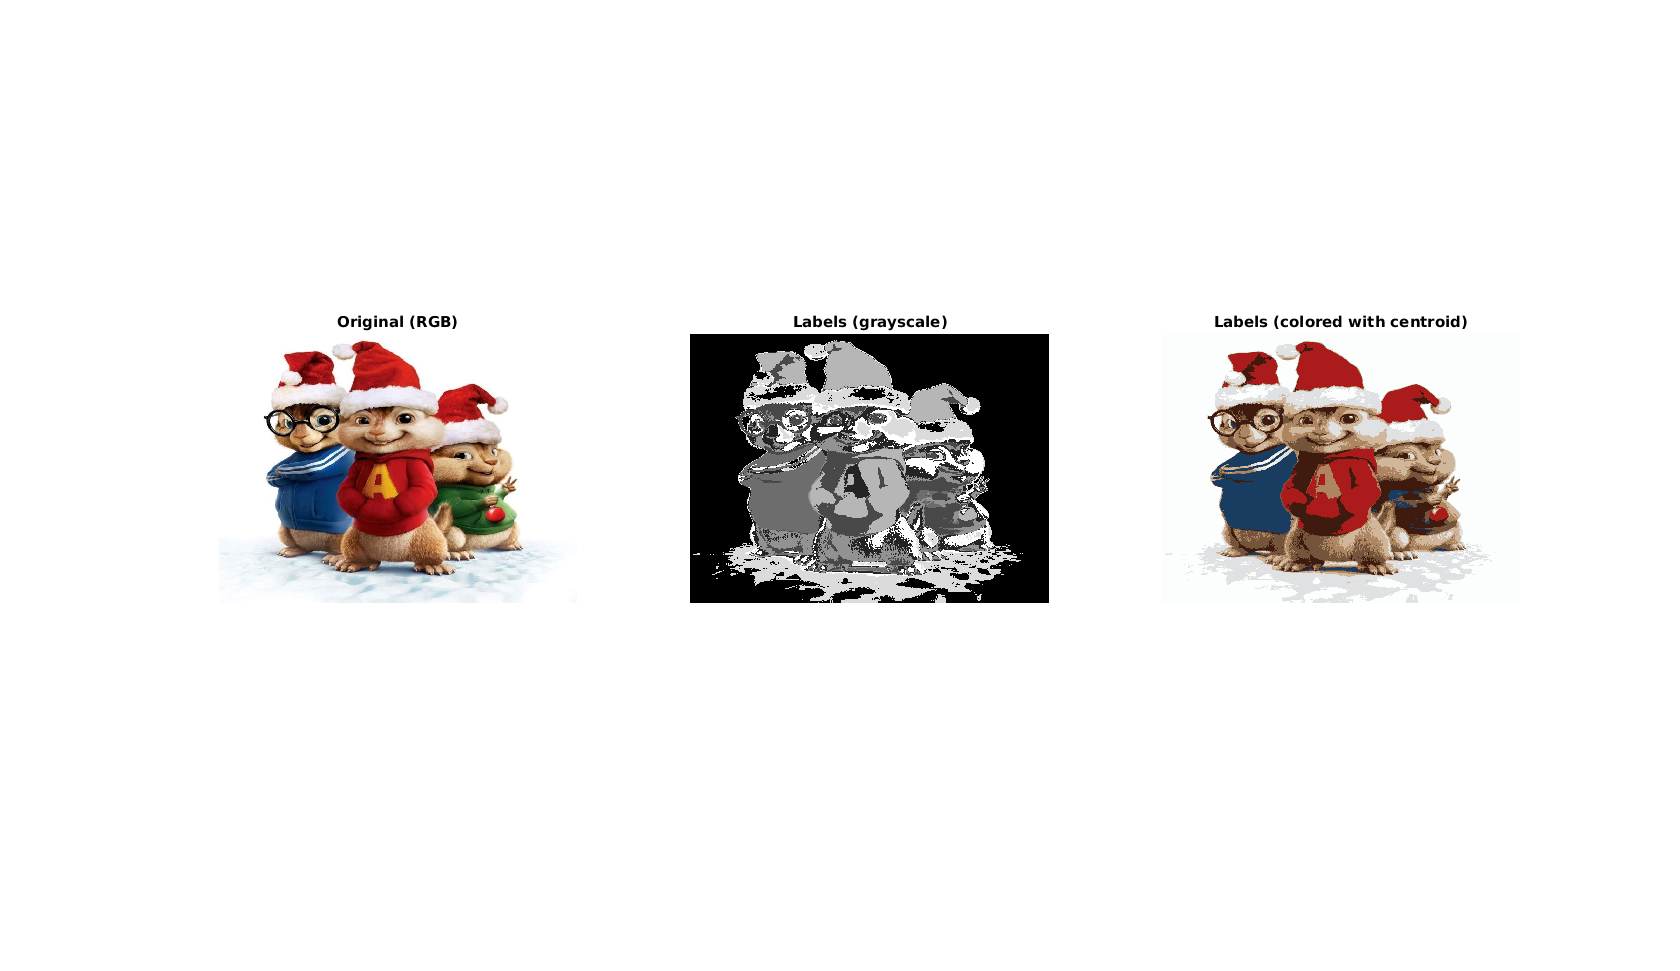
\includegraphics[trim={50px 250px 50px 170px},clip,width=\textwidth]{img/kmeans/alwin2_k8_no_spatial.png}
\caption{Segmentation of \texttt{alwin2.jpg} with K-means (K = 8)}
\label{fig:alwin2-k8-no-spatial}
\end{figure}

The algorithm may or may not be deterministic depending upon the choice of
parameters. The default start method, \emph{kmeans++}, is
stochastic (although it
applies a certain heuristic in order to have the initial clusters as far
apart from each other as possible). The other named methods (\emph{sample}, \emph{uniform},
\emph{cluster}) are stochastic as well. There is an additional start
method which consists in accepting from the user a matrix with the initial
clusters' centroids. Should these clusters be decided deterministically
the algorithm will perform the same steps at each run. For the purpose
of our analysis we will stick to \emph{kmeans++}.

We can see how the results can (and will, generally) be different between
successive runs of the algorithm with the same
arguments and the same image in figure
\ref{fig:animals-k10-no-spatial-differences}.

Of course, when using any of the stochastic methods we can force the results to be the
same at each run by fixing the seed of the Random Number Generator (RNG).

\begin{figure}[hbt]
\centering
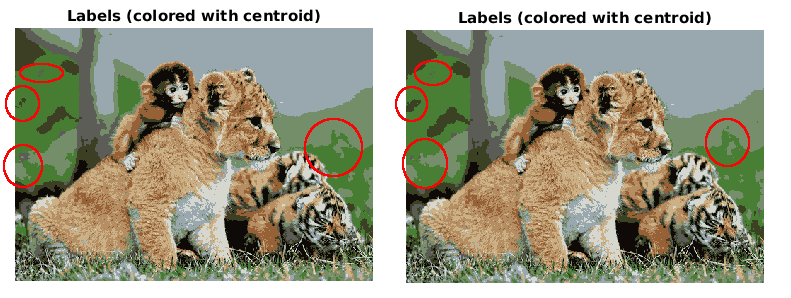
\includegraphics[width=\textwidth]{img/kmeans/animals_k10_no_spatial_differences.png}
\caption[Results of successive runs of the k-means algorithm for \texttt{animals.jpg} with K=10]
{Results of successive runs of the k-means algorithm for \texttt{animals.jpg} with K=10. The most noticeable differences are marked with a red circle.}
\label{fig:animals-k10-no-spatial-differences}
\end{figure}

In order to check whether the results are the same when applying transformations to the
image, and bearing in mind the previous explanation, we need to fix the state of the RNG
(otherwise the results would be different no matter there is a transformation or not).
Even doing so we can anticipate that we will obtain different results since these
transformations have an influence over the initialization method (whenever it is one of the
named stochastic methods). In the case of scaling the image this becomes obvious when we
take the limit case and scale the image down to just one pixel (e.g. the average of all the
pixels in the image). In general scaling down the image removes details and can result in
redundant clusters and/or less noisy labels. On the other hand scaling the image up can
magnify noisy sections of the
image that can fool the algorithm into assigning a cluster to those spurious regions.
Finally rotating the image has an impact on the order in which
the data is presented to the algorithm.

In figure \ref{fig:kmeans-geometric-transformations} we can appreciate that these
geometrical transformations have indeed an impact over the outcome of the algorithm. However it is
worth noticing that under reasonable circumstances (i.e. no extreme or contrived
transformations and not too much noise) the results are fairly similar from a qualitative
point of view. Perhaps the most significant change is seen when we scale down the image to
0.25 of the original dimensions (i.e. 16 times less area), since the label assigment to
the lion and the grass section is not so noisy.

\begin{figure}[hbt]
	\centering
	\begin{subfigure}[t]{0.3 \textwidth}
		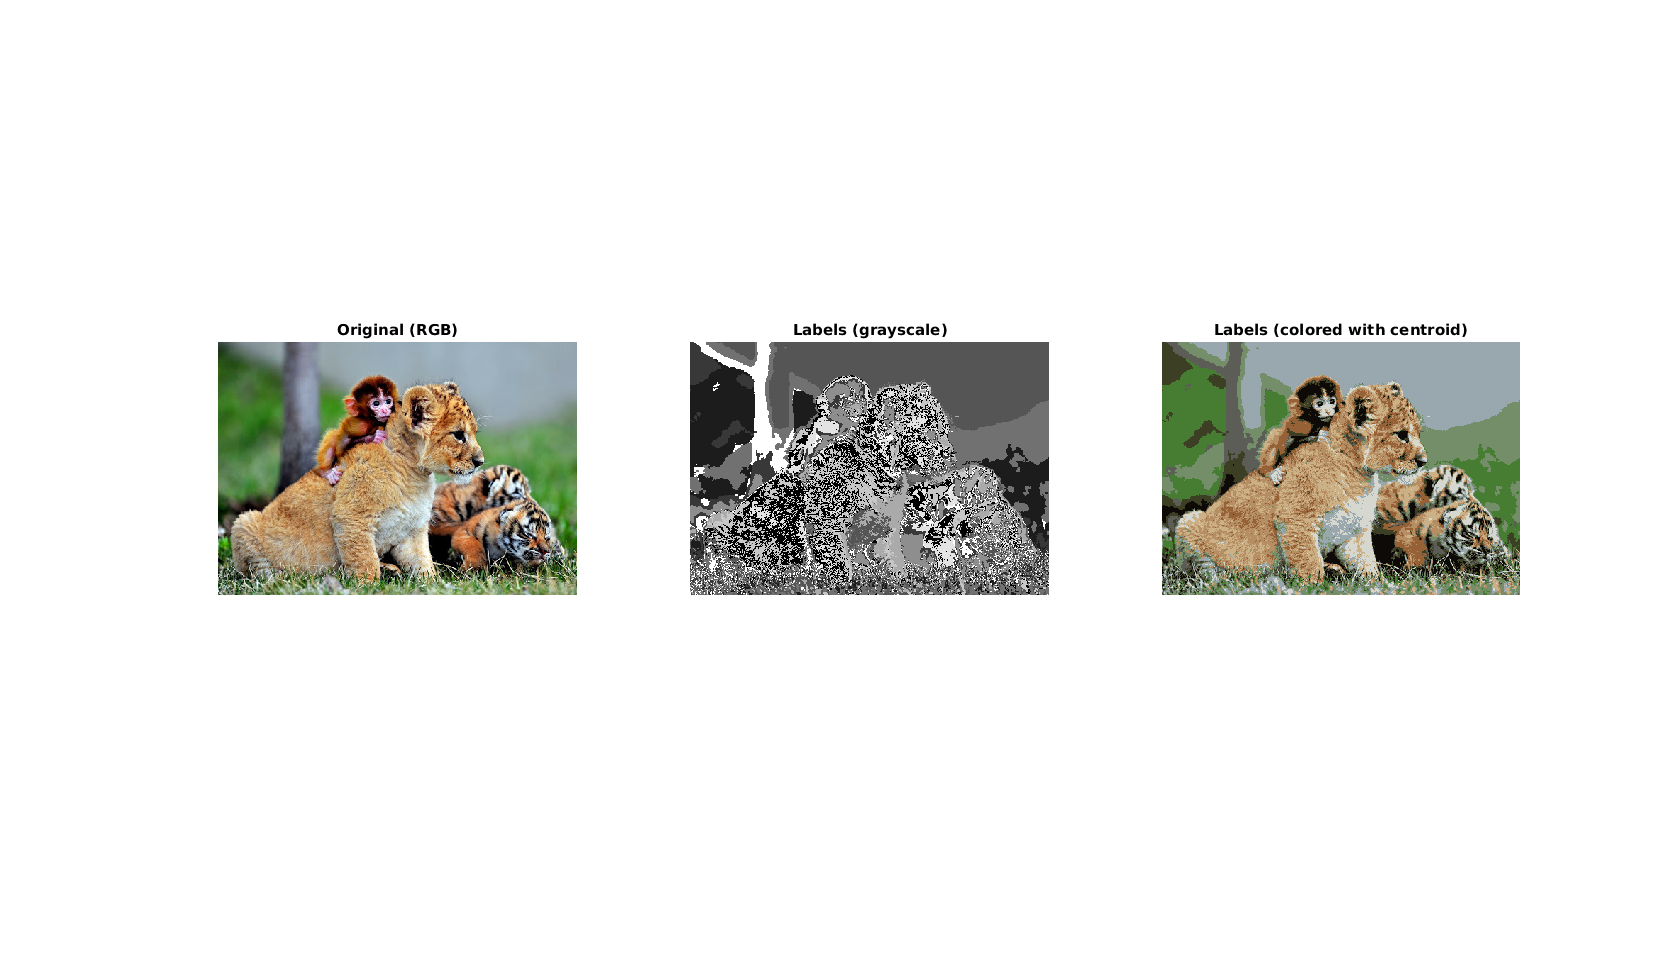
\includegraphics[trim={825px 250px 50px 220px},clip,width=\textwidth]{img/kmeans/animals_k10_no_spatial.png}
		\caption{Original}
		\label{fig:kmeans-geometric-transformations-original}
	\end{subfigure}
	
	\begin{subfigure}[t]{0.3 \textwidth}
		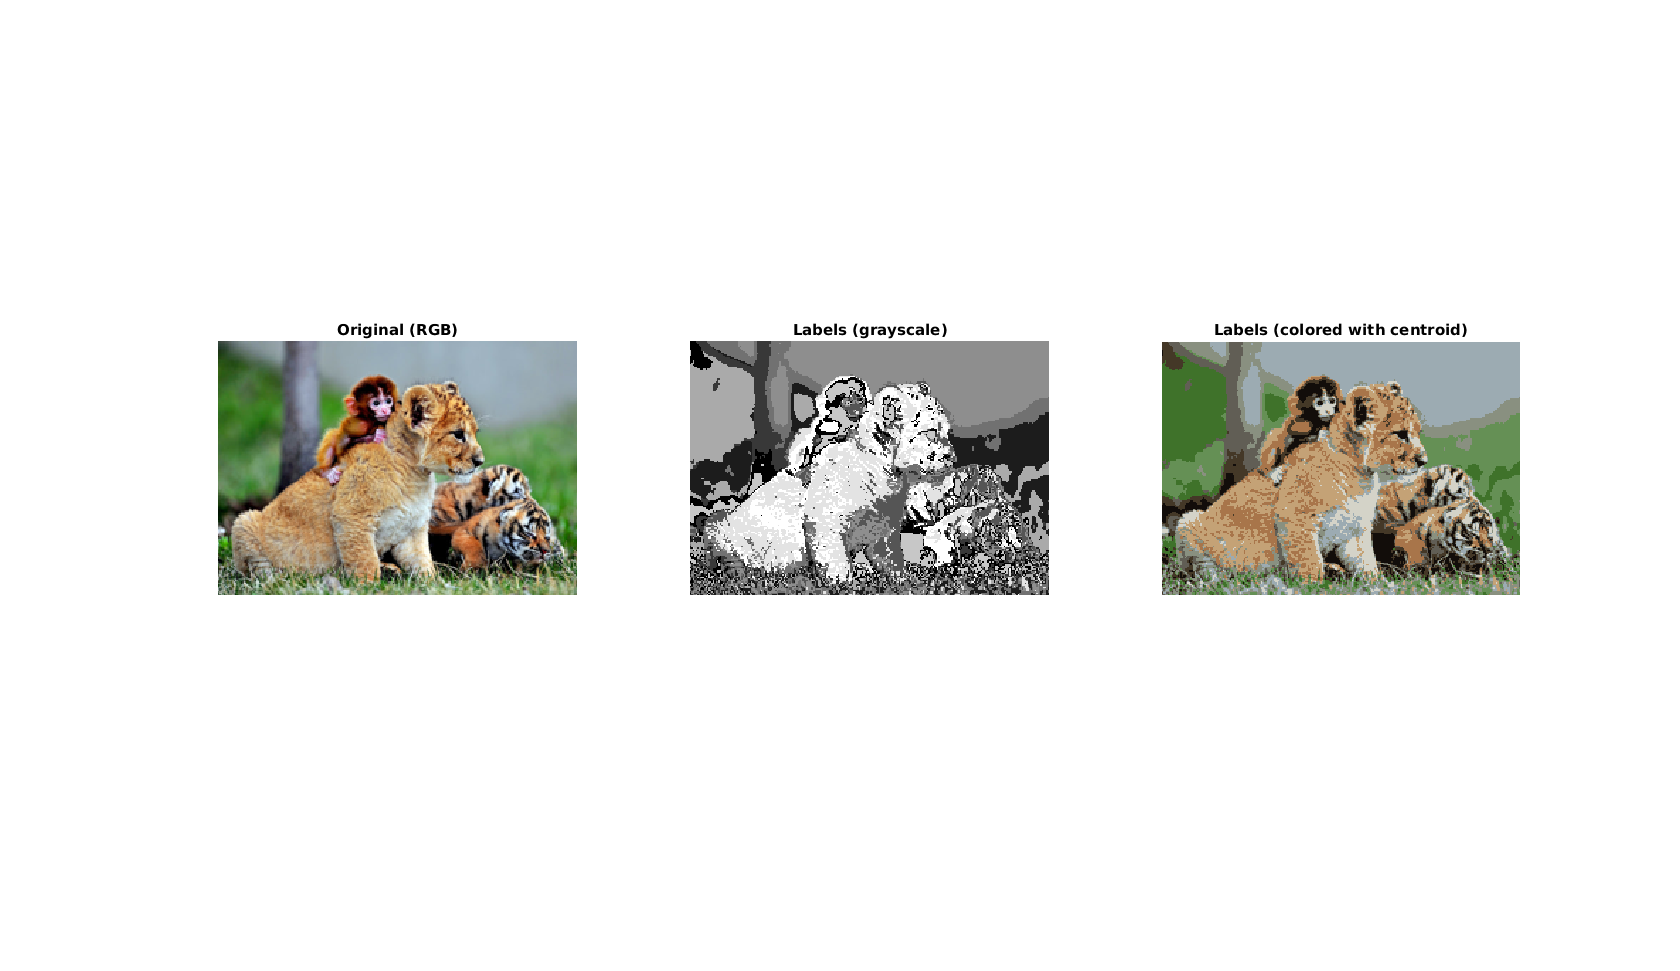
\includegraphics[trim={825px 250px 50px 220px},clip,width=\textwidth]{img/kmeans/animals_k10_no_spatial_scaled_down.png}
		\caption{Scaled down (s=0.5)}
		\label{fig:kmeans-geometric-transformations-scaled-down}
	\end{subfigure}
	~
	\begin{subfigure}[t]{0.3 \textwidth}
		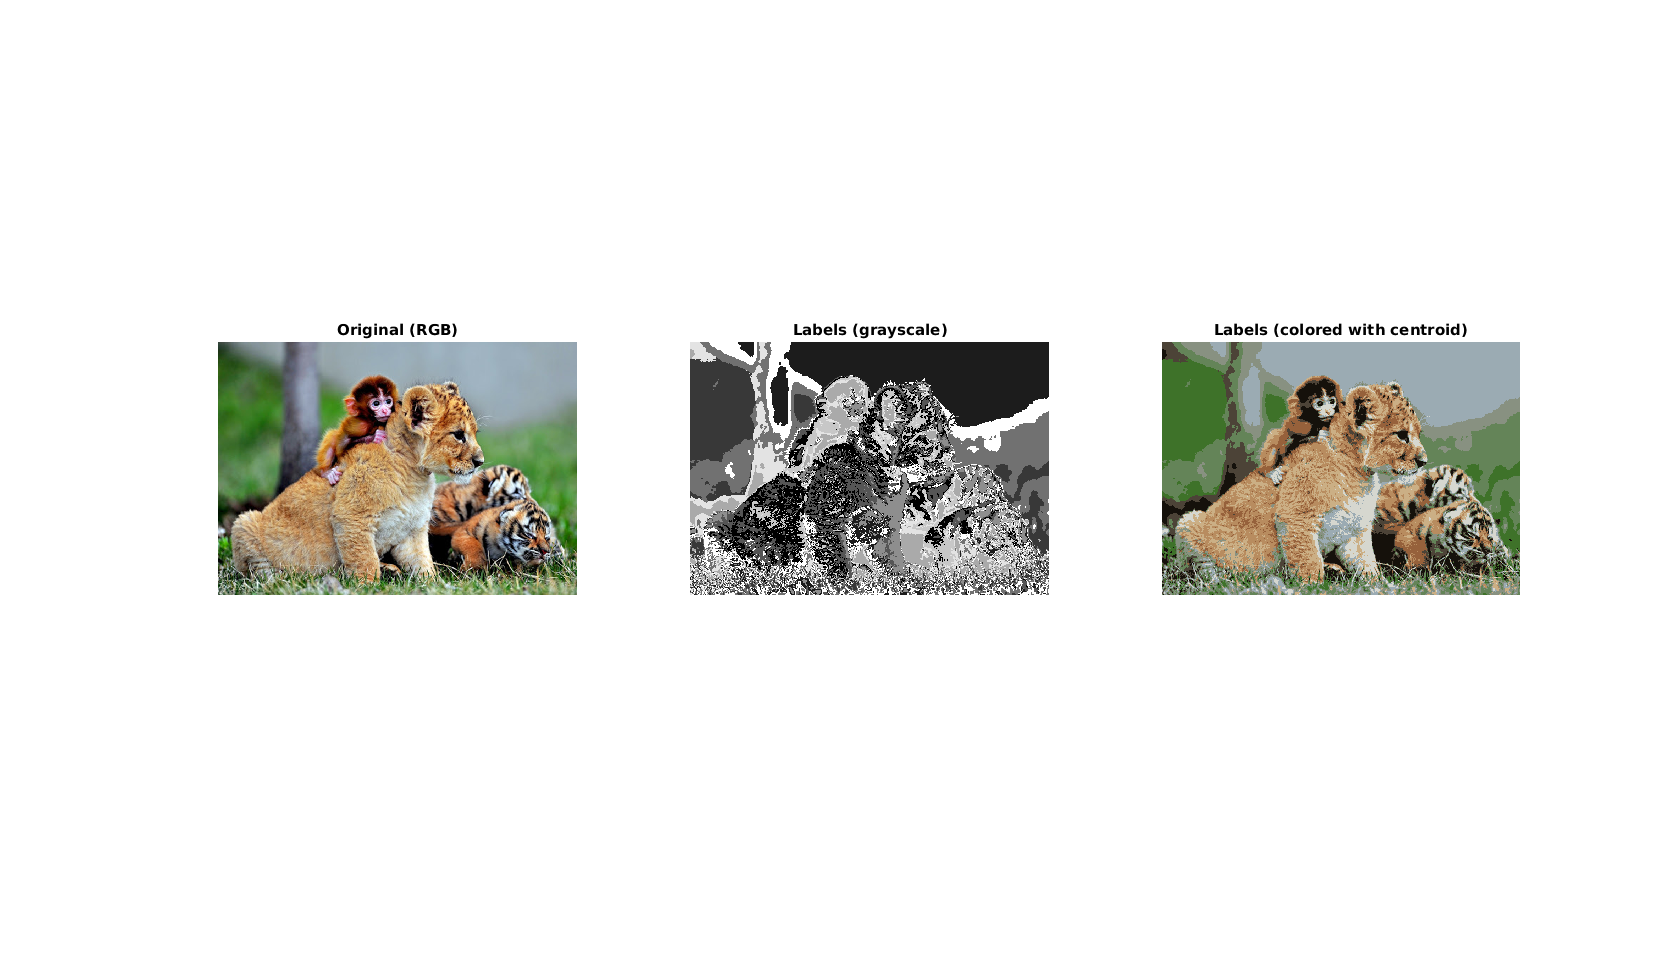
\includegraphics[trim={825px 250px 50px 220px},clip,width=\textwidth]{img/kmeans/animals_k10_no_spatial_scaled_up.png}
		\caption{Scaled up (s=2)}
		\label{fig:kmeans-geometric-transformations-scaled-up}
	\end{subfigure}
	~
	\begin{subfigure}[t]{0.3 \textwidth}
		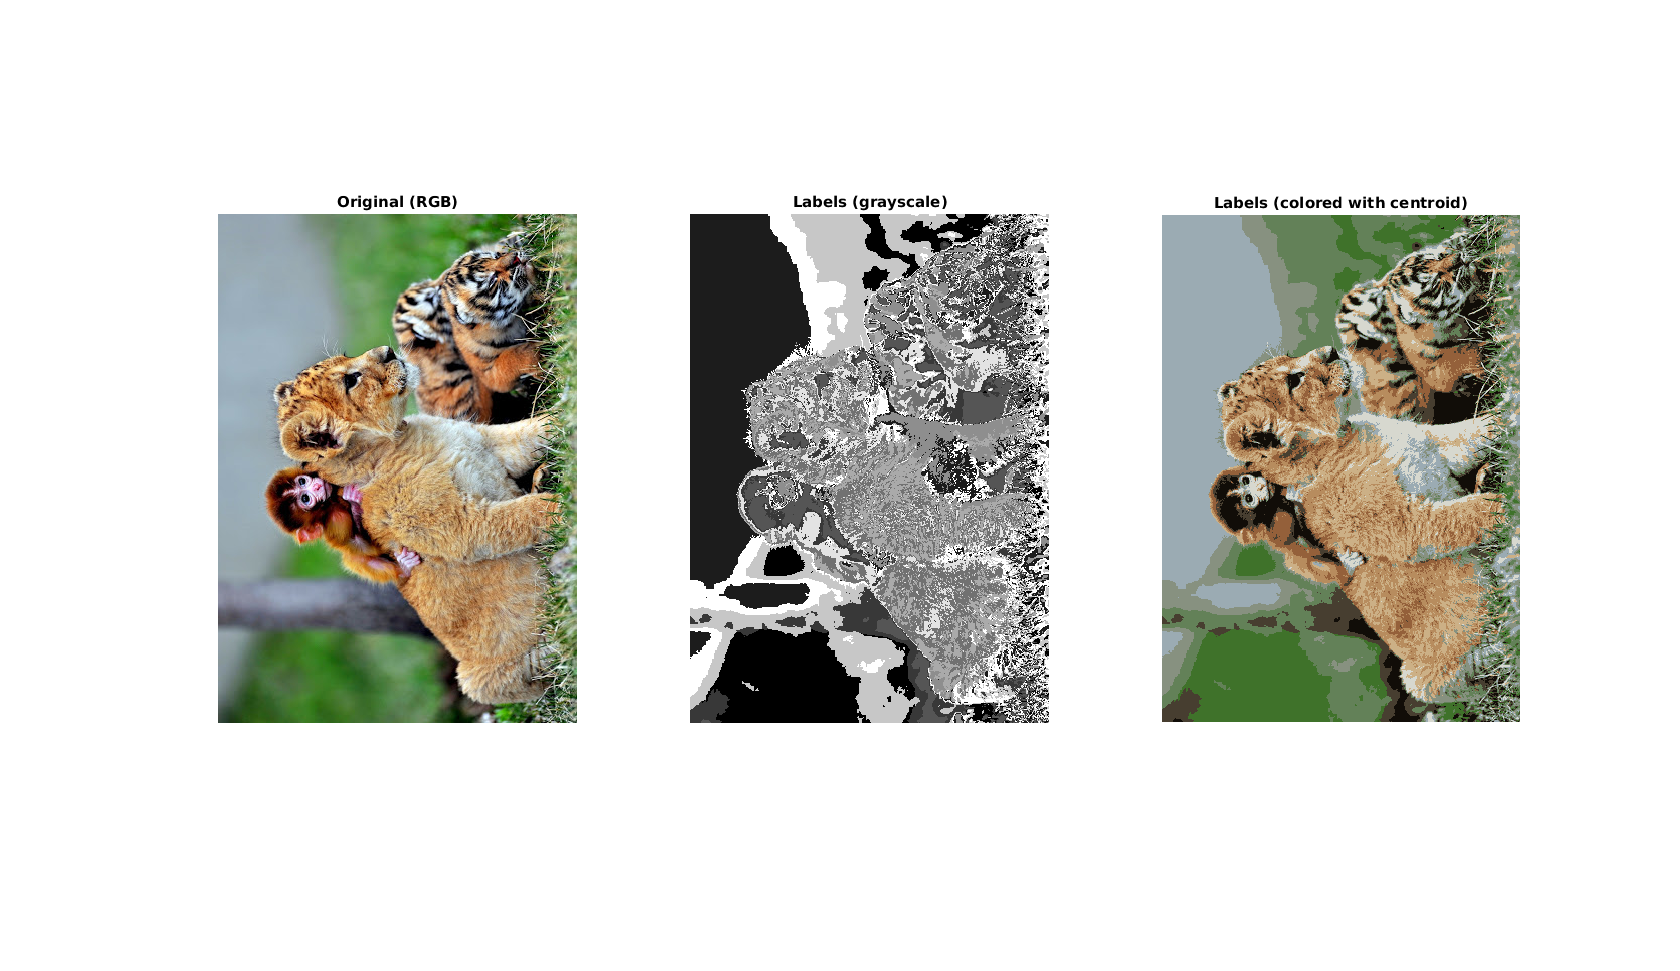
\includegraphics[trim={825px 250px 50px 150px},clip,width=\textwidth]{img/kmeans/animals_k10_no_spatial_rotated.png}
		\caption{Rotated}
		\label{fig:kmeans-geometric-transformations-rotated}
	\end{subfigure}
	
	\caption{Comparison of k-means' (K=10) results after applying geometric transformations}
	\label{fig:kmeans-geometric-transformations}
\end{figure}

\subsection{Adding spatial information to the k-means algorithm}

In figure \ref{fig:animals-k10-spatial} and \ref{fig:animals-k5-spatial} we can
see what the results for \texttt{animals.jpg} when we include the spatial coordinates in
the data passed to the k-means algorithm. We can see that now the pixel
coordinates has a significant weight when determining the cluster it belongs to. This helps
to fight some of the problems we had before: now the labels assigned to the grass section
do not seem so erratic and spurious.

On the other hand we can see as a disadvantage that
large entities being cut asunder whenever they are too large (like the baby lion
in the middle). Not only that, now the size of the image have a great weight over the
segmentation process. The bigger the image the more will it resemble a Voronoi diagram
rather than an image segmented by colors. Figures \ref{fig:alwin2-k8-spatial}
and \ref{fig:bigbangfamily-k8-spatial} illustrates this even better.

\begin{figure}[hbt]
\centering
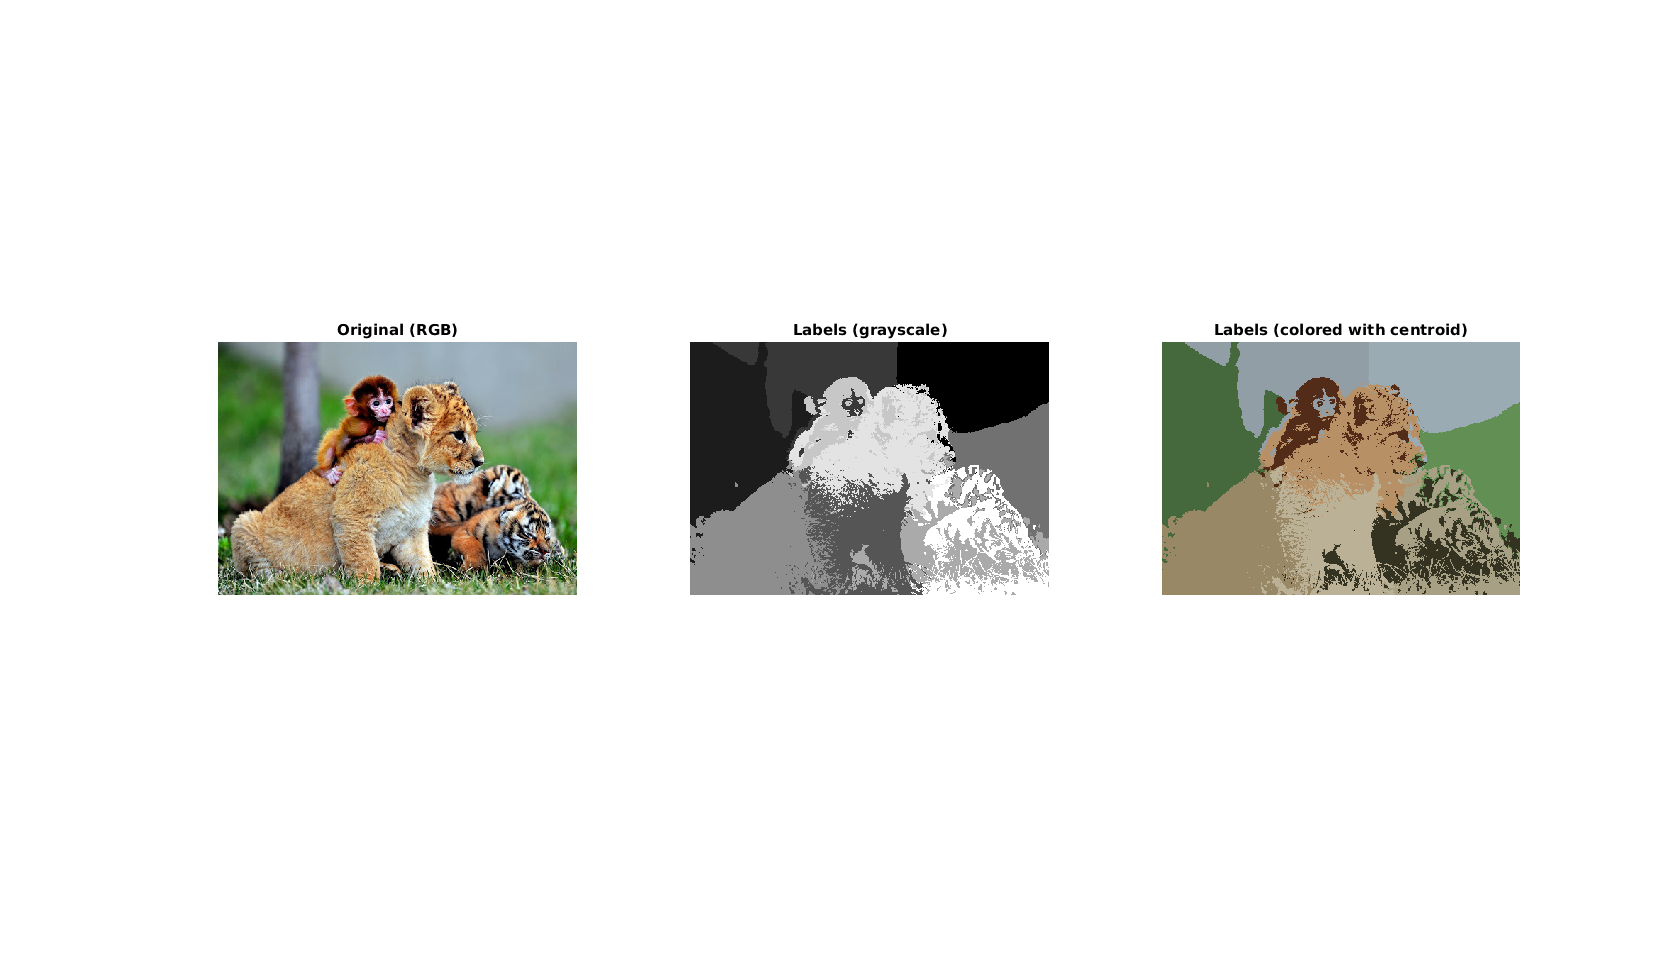
\includegraphics[trim={50px 250px 50px 225px},clip,width=\textwidth]{img/kmeans/animals_k10_spatial.png}
\caption{Segmentation of \texttt{animals.jpg} with K-means (K = 10) and spatial coordinates}
\label{fig:animals-k10-spatial}
\end{figure}

\begin{figure}[hbt]
\centering
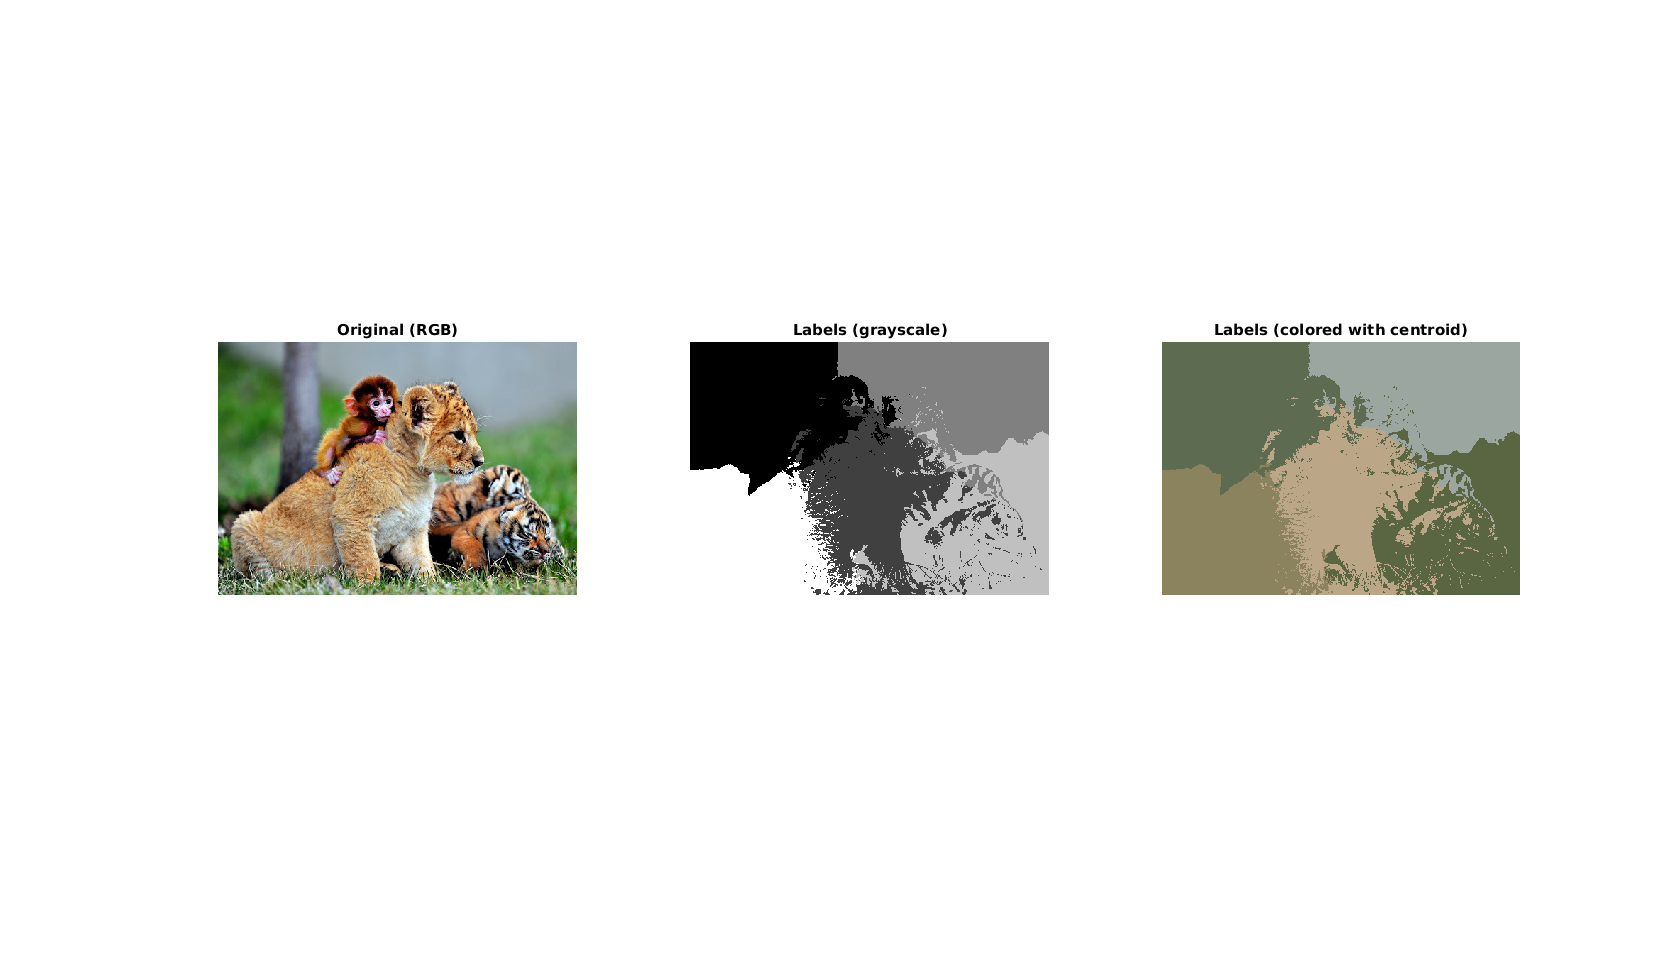
\includegraphics[trim={50px 250px 50px 225px},clip,width=\textwidth]{img/kmeans/animals_k5_spatial.png}
\caption{Segmentation of \texttt{animals.jpg} with K-means (K = 5) and spatial coordinates}
\label{fig:animals-k5-spatial}
\end{figure}

\begin{figure}[hbt]
\centering
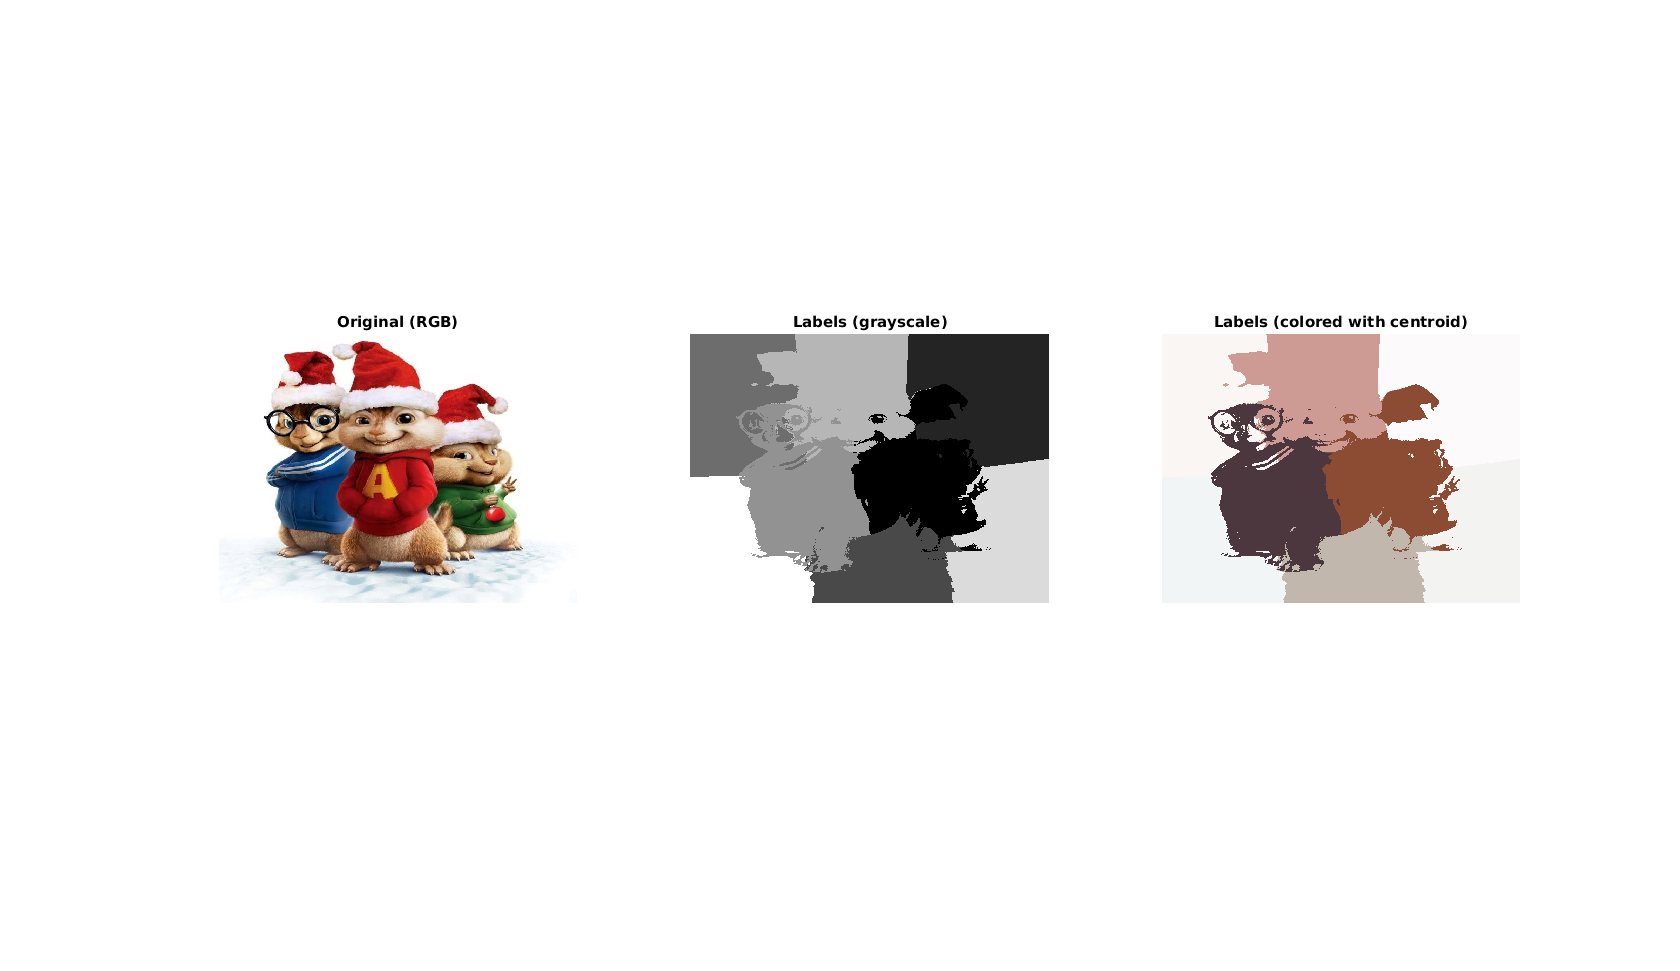
\includegraphics[trim={50px 250px 50px 170px},clip,width=\textwidth]{img/kmeans/alwin2_k8_spatial.png}
\caption{Segmentation of \texttt{alwin2.jpg} with K-means (K = 8) and spatial coordinates}
\label{fig:alwin2-k8-spatial}
\end{figure}

\begin{figure}[hbt]
\centering
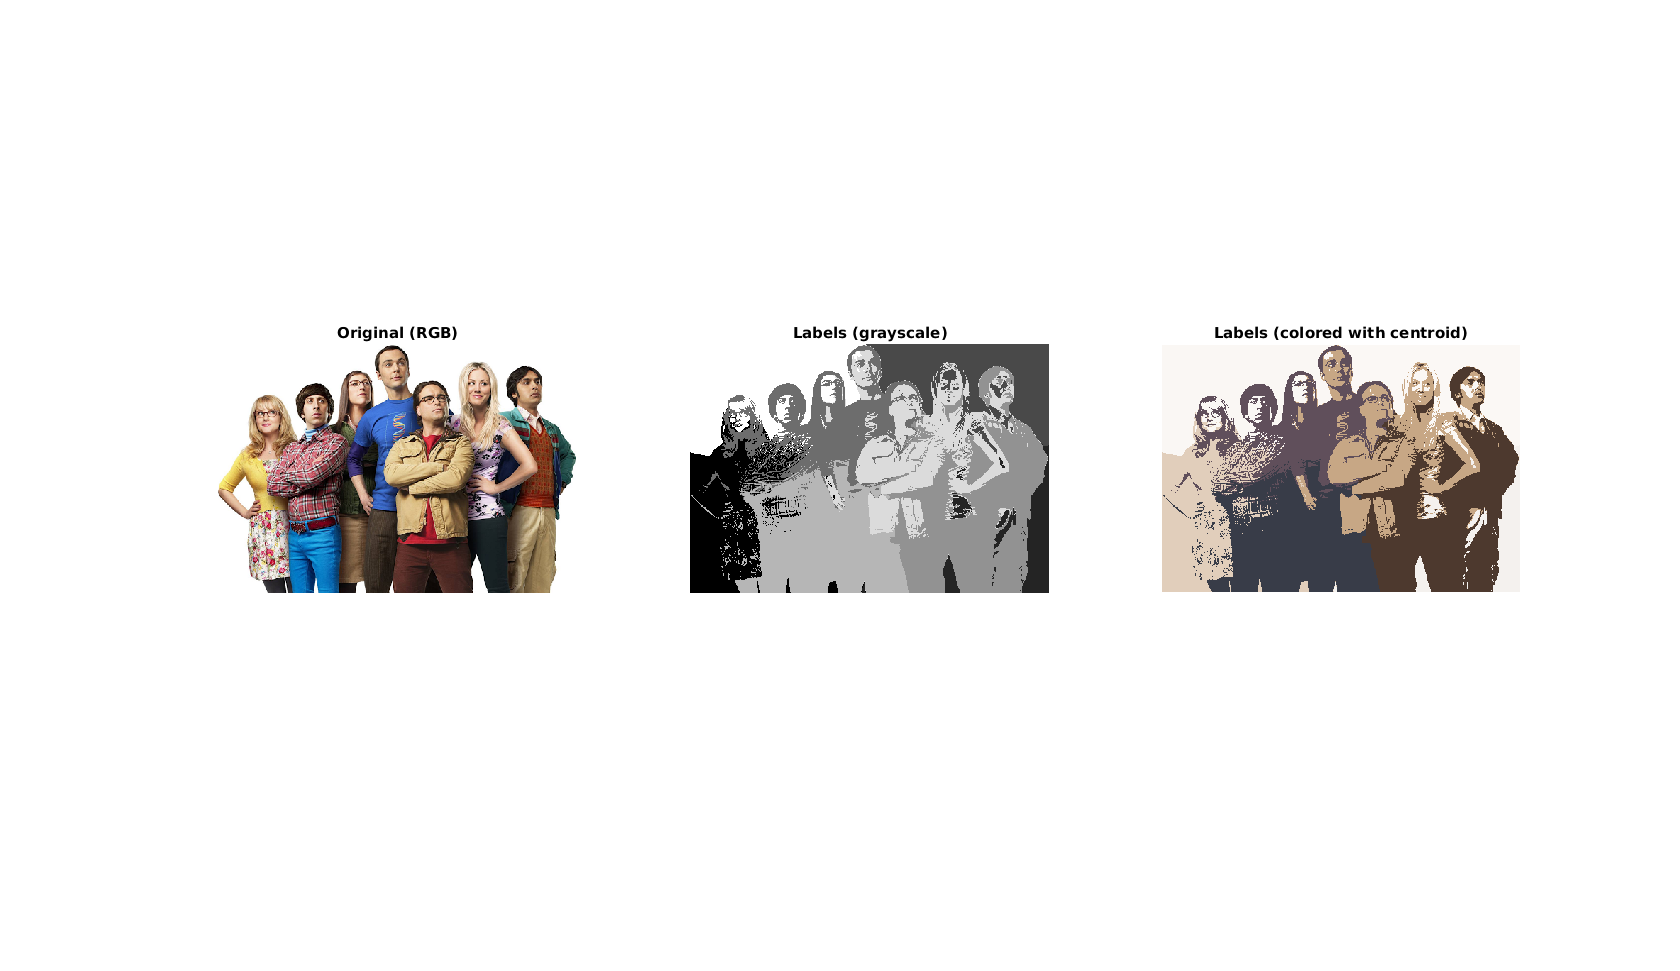
\includegraphics[trim={50px 250px 50px 200px},clip,width=\textwidth]{img/kmeans/bigbangfamily_k8_spatial.png}
\caption{Segmentation of \texttt{bigbangfamily.png} with K-means (K = 8) and spatial coordinates}
\label{fig:bigbangfamily-k8-spatial}
\end{figure}

The spatial coordinates can help to discriminate between two entities
that have similar colors but are distant from each other. This means that the number of
clusters would ideally be chosen to match the number of expected single-color compact
entities in the image, instead
of the number of colors. In general this is difficult.
Moreover, when using Euclidean distance with k-means
we are assuming spherical clusters which in general do not adjust well to the figures in
our image (e.g. the elongated shape of the lion).

Now the size of the image has to be chosen well. Scaling
down \texttt{animals.jpg} before applying k-means with K=10 and spatial coordinates,
as shown in figure
\ref{fig:animals-k10-spatial-scaled-down},
renders a much better segmentation than that showed in figure \ref{fig:animals-k10-spatial}.
One could think
that the clusters are even better than in figure \ref{fig:animals-k10-no-spatial} since
the baby lion is segmented much more uniformly and the grass region presents less noise now
that the spatial coordinates are taken into account.

\begin{figure}[hbt]
\centering
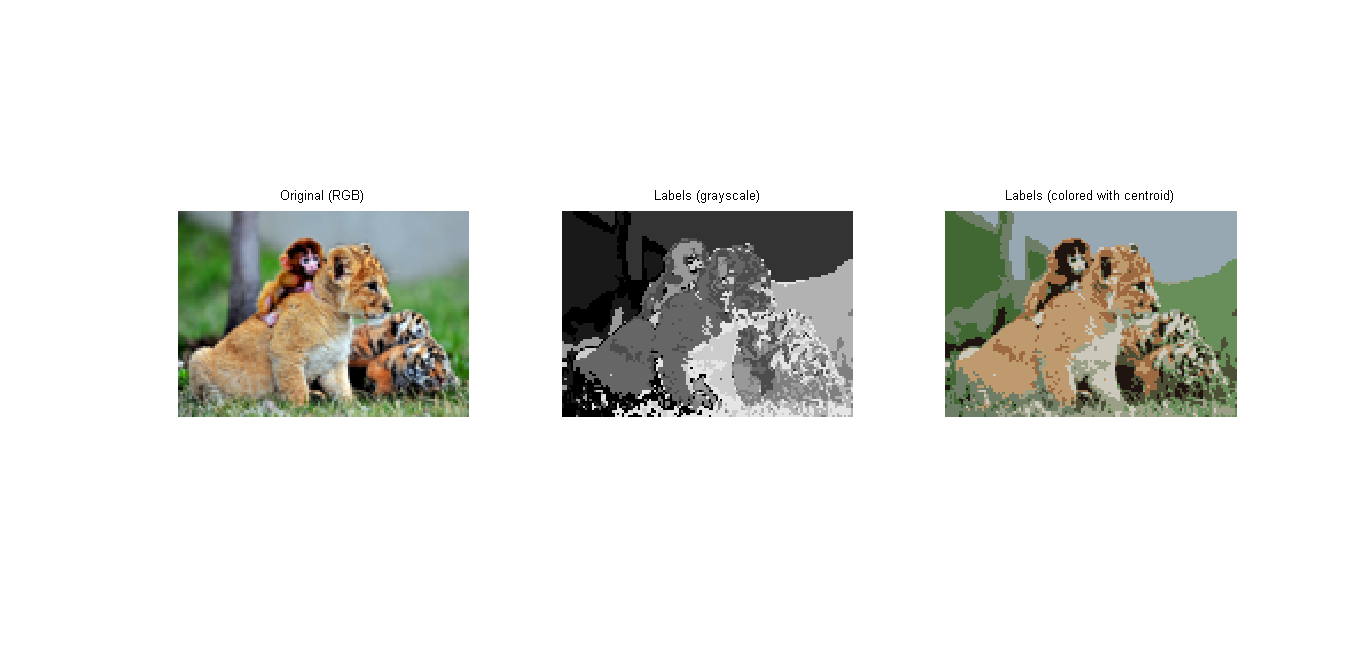
\includegraphics[trim={50px 150px 50px 125px},clip,width=\textwidth]{img/kmeans/animals_k10_scaled_down_spatial.png}
\caption{Segmentation of \texttt{animals.jpg} (scaled down, s=0.25) with K-means (K = 10) and spatial coordinates}
\label{fig:animals-k10-spatial-scaled-down}
\end{figure}

\subsection{Additional observations}

Alternatively, instead of scaling the image down, we could introduce a
variant of the Euclidean distance that weights differently the distance
in the color space and the geometrical distance. In this same line of thought one
could even weight differently the difference of each attribute without caring if
it is a color attribute or a spatial one (e.g. giving
more importance to the red channel). Other possibilities include using
color spaces like CIEL*a*b that take into account the human perception and in which
the distances are more meaningful in a perceptual sense. In this color space the
L* channel represents the luminosity and can be thrown away if our purpose is to
segment by perceived color minimizing
the impact of light changes. All these ideas can be applied to the following algorithm
we will cover (Mean-shift) as well, although they will not be covered in this document.

\FloatBarrier